\subsection{\gls{spade} inputs}
The inputs to our design flow are details of the \gls{ibc} application, other applications sharing the platform, given platform allocation for the \gls{ibc} application and camera characteristics, e.g.\ \gls{fps}. These should be compliant with the application and platform models. Note that the details of the other applications sharing the platform are not relevant for a composable platform such as \gls{compsoc}. 

\subsection{Formal modelling: application and platform models}
A typical \gls{ibc} application model of an \gls{lkas} is shown in Fig.~\ref{fig:ch5_SADF}(a).
The details of this model have already been explained in Section~\ref{sec:ch5_MoC}.
Task-level \gls{wcet} profiling is required to compute the \glspl{wcet} on the \gls{compsoc} platform.
The platform is modelled as a platform graph as described in Section~\ref{sec:compsoc}. 

\subsection{Analysis and design}
\subsubsection{System mapping} 
We first describe the system mapping, i.e., binding and scheduling, of our \gls{ibc} application model to the platform.
Fig.~\ref{fig:ch5_SADFeg} illustrates three workload scenarios and their possible platform mapping.\footnote{The indices for the RoIP actors are omitted for readability. The functionality of the different RoIP actors is the same.} Fig.~\ref{fig:ch5_SADFeg}(a), (c), and (e) model the dataflow graphs for different workloads (note the absence of self-loops for the RoIP actors) and Fig.~\ref{fig:ch5_SADFeg}(b), (d) and (f) show their corresponding mappings and execution on two or three processor tiles \emph{P}$_i$. Having more processor tiles means that we can reduce $h$ and $\tau$ by parallel execution of the sensing tasks.

\begin{figure}
    \centering
    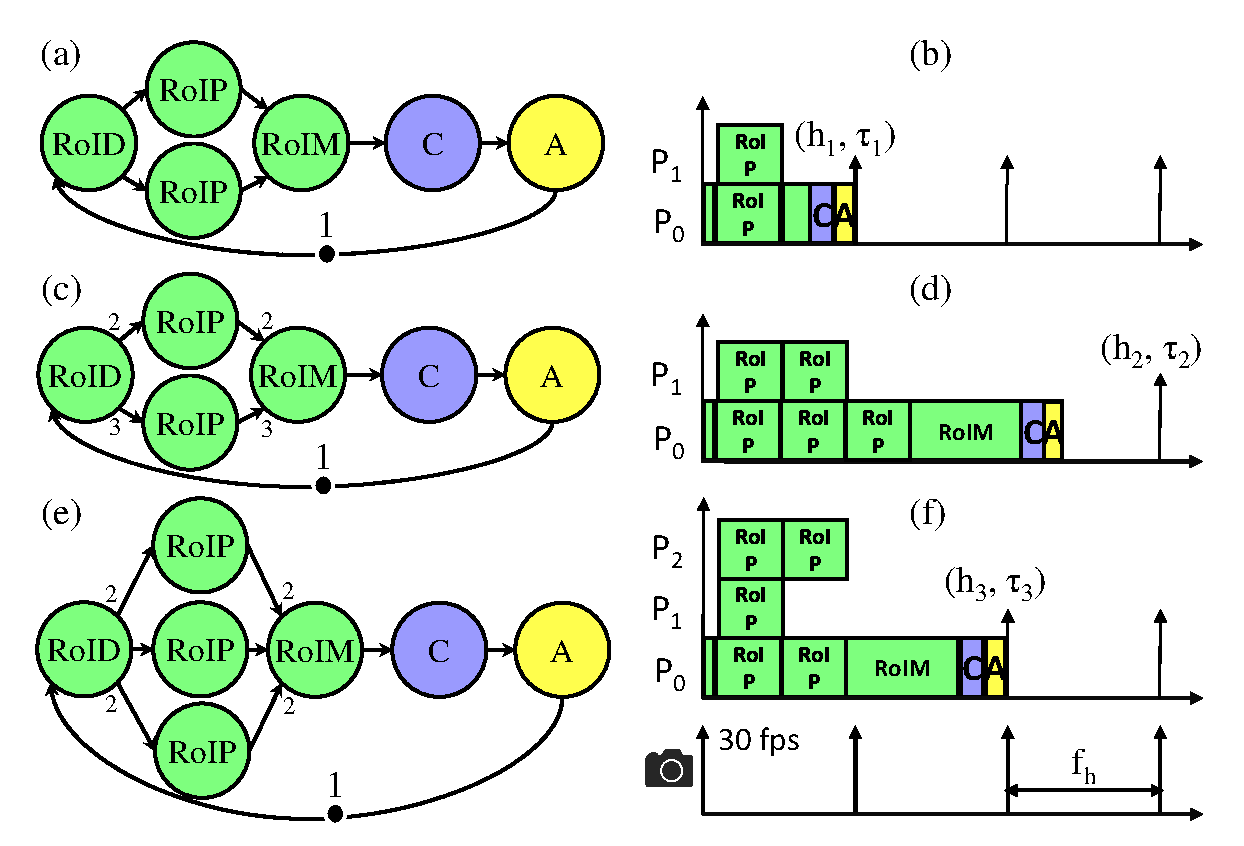
\includegraphics[scale=0.5]{images/SADFeg.eps}
    \caption{Illustration of workload variations and platform mapping.}
    \label{fig:ch5_SADFeg}
    %\vspace{-2em}
\end{figure}

System mapping refers to the mapping of application tasks (modelled as an \gls{sadf} model) to the platform. An application can have multiple mapping options for a given platform allocation. For example, in Fig.~\ref{fig:ch5_SADFeg}(c) and (e), the given platform allocation is two and three processor tiles respectively (visible in the number of RoIP actors) for the same workload (5 \gls{roi}).

\subsubsection{Timing analysis: relation between dataflow analysis and control design}
\label{sec:ch5_relation}
The inverse throughput of the mapped binding-aware \gls{sdfg}  $\bindingAwareSDFG{i}$ for scenario sequence $\scenario_i^\omega$ gives the sensor-to-actuator delay $\tau_{i}$; the sampling period $h_i$ can be derived from the sensor-to-actuator delay and expressed in terms of the frame arrival period $\fh$, i.e.,
\begin{eqnarray}
\tau_{i}= \frac{1}{\FnThroughput(\scenario_i^\omega)},\ h_{i}=\lceil \frac{\tau_{i}}{\fh}\rceil \fh.\
\nonumber
\end{eqnarray}

The timing parameters for the three mapped workload scenarios in Fig.~\ref{fig:ch5_SADFeg} are obtained as follows: 
\begin{eqnarray}
\tau_i = \actorET_d+(\max\limits_i^{\numCoresAvailable} y_i)\times \actorET_p+\actorET_m+\actorET_c+\actorET_a,\ h_i= \lceil \frac{\tau_i}{\fh}\rceil \fh,\nonumber
\end{eqnarray}
 where ${\numCoresAvailable}$ represents the total number of available (or allocated) processors. Assume $\fh=\frac{1}{30}$s for a camera with 30 fps and $\actorET_m=7\times(\sum\limits_i^{\numCoresAvailable} y_i)$. Cost of communicating data between processors is assumed to be part of the actor execution times $\actorET_i$; if meaningful, such cost could be made explicit, but for simplicity, we do not do so. For our example shown in Fig.~\ref{fig:ch5_SADFeg}:
\begin{eqnarray}
\noindent\tau_1 &=& 5+1\times10+7\times (1+1)+2+2=33 \text{ms},\nonumber\\
\tau_2 &=& 5+3\times10+7\times (2+3)+2+2=74 \text{ms},\nonumber\\
\tau_3 &=& 5+2\times10+7\times(2+1+2)+2+2=64 \text{ms},\nonumber
\end{eqnarray}
and $h_1=\fh,\ h_2=3\fh,\ h_3=2\fh$. 

\subsubsection{Control design}
Once we obtain $\tau_{i}$ and $h_{i}$ for mapped workload scenario $\workloadScenario$, they are then used for the discrete-time controller implementation as described in Section~\ref{sec:ch5_embeddedIBC} and for designing the controller gains. Further, the timing parameters are a part of the control configuration as defined in Section~\ref{sec:ch5_ch5_control law}. Any  state-of-the-art control design method can be used for this design. 

\subsubsection{Optimal system-scenario identification}~\label{sec:ch5_ch5_sys_scenario}
It is possible for multiple workload scenarios to have the same sampling period due to implementation constraints like platform allocation and camera frame rate. For example, for the workload scenario represented in Fig~\ref{fig:ch5_SADFeg} (a) with ($h_1,\tau_1$), the number of \gls{roi}, \#\gls{roi} $=2$. However, even for the workload scenario with \#\gls{roi} $=1$ mapped to two processors, we would have the same timing parameters ($h_1,\tau_1$) since the tasks would have to execute sequentially on one processor. Similarly, for the workload scenario in Fig~\ref{fig:ch5_SADFeg}~(c), we would have the same timing parameters for \#\gls{roi} 5 and 6.

A system scenario $\sysScenario$ abstracts multiple workload scenarios $\workloadScenario$ such that for $h_s=n\times \fh$ for some $n>0,\ (h_s-\fh) < h_i \leq h_s$ and $\tau_i \leq \tau_s$.
Only system scenarios are then considered for defining the control configuration and for platform implementation.

The system scenarios we consider for this case are $\{s_1=(\fh,33),\ s_2=(2\fh,57),\ s_3=s_{wc}=(3\fh,74)\}\ ms$.
The worst-case system scenario $s_{wc}$ is the scenario corresponding to the worst-case image workload (which in our case is 6 \glspl{roi}). The other two scenarios correspond to workloads of 1 or 2 resp.\ 3 or 4 \glspl{roi}. The workload with 5 \glspl{roi} is part of the worst-case system scenario.

Once we identify the timing parameters for our system scenarios, we design the controller and compute $(\Kgain_{\sysScenario},\ \Fgain_{\sysScenario})$ for each system scenario $\sysScenario$.
Then, the controller stability needs to be guaranteed for the system scenario switching (as explained in Section \ref{sec:ch5_controller_stability}). If the controller stability is guaranteed, then we can proceed with the implementation. Otherwise, we need to choose a different (sub)set of system scenarios for which the system scenario switching is stable. For the scope of this chapter, this is done by a brute-force approach. In case we cannot identify any stable switching (sub)set of system scenarios, we revert to the design with the worst-case scenario $s_{wc}$ as the single system scenario.

\subsection{Implementation and runtime reconfiguration mechanism}
The optimal system scenarios are identified and their corresponding control and mapping configurations are stored as a \gls{lut} in platform memory for runtime implementation.
During runtime, for every arriving input image frame, we compute the workload (e.g.\ through an image pre-processing step) and choose the correct system scenario associated with this workload from the \gls{lut}. 
Controller and mapping configurations of the corresponding system scenario are loaded from the \gls{lut}. A scheduler then reconfigures the mapping, the time-triggering of the actuation task and the controller gain parameters based on the chosen system scenario. The overhead cost for this reconfiguration has already been considered in our
analysis model as a time cost in the start of sensing task (e.g.\ along with the actor RoID in Fig.~\ref{fig:ch5_SADF}).

\section{Simulation results}
In this section, we analyse the performance of our basic \gls{spade} flow through simulations. We first analyse the impact of workload variations and then compare our approach to a state-of-the-art pipelined control implementation.

\subsection{Impact of workload variations}
\label{sec:ch5_impact_workload}
\begin{figure}
            \centerline{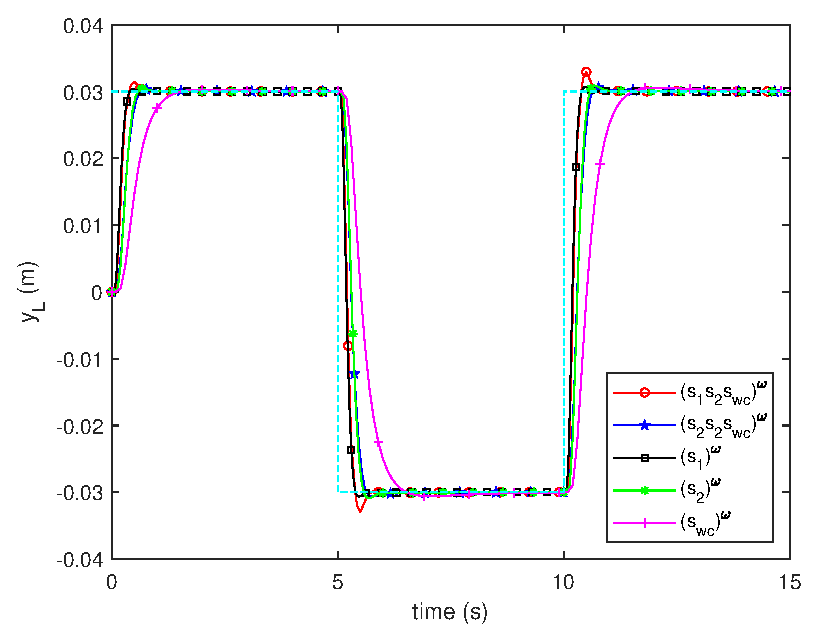
\includegraphics[width=0.6\textwidth]{images/res_DSD.eps}}
            \vspace{-1ex}
            \caption{Controller performance: comparison of switching subsystems with worst-case $s_{wc}$}
            \label{fig:ch5_results}
            \vspace{-2ex}
\end{figure}
The \gls{qoc} provided by an \gls{ibc} system depends on the nature of workload variation encountered by the application resulting in different switching sequences. We simulate the \gls{lkas} controller performance for various system scenario switching sequences with 2, 4, and 5 \glspl{roi} and sampling periods $h_1=0.033$s, $h_2=0.066$s, and $h_{wc}=0.100$s for the corresponding system scenarios $s_1,\ s_2,$ and $s_{wc}$, respectively, as shown in Fig.~\ref{fig:ch5_results}.
We assume that there are 6 \glspl{roi} in the worst-case.
We observe that our switching designs of \gls{spade} (plot $(s_1 s_2 s_{wc})^\omega$ and $(s_2 s_2 s_{wc})^\omega$) have better \gls{qoc} (low \gls{mse}) than the worst-case sampling period based design (see plot $(s_{wc})^\omega$) in Fig.~\ref{fig:ch5_results}. An example switching sequence is illustrated in Fig.~\ref{fig:ch5_result2}(a). We see that the effective resource utilisation for each sampling period is improved (with less idling) with respect to the worst-case based design in Fig.~\ref{fig:ch5_result2}(b). 
\begin{figure}
            \centerline{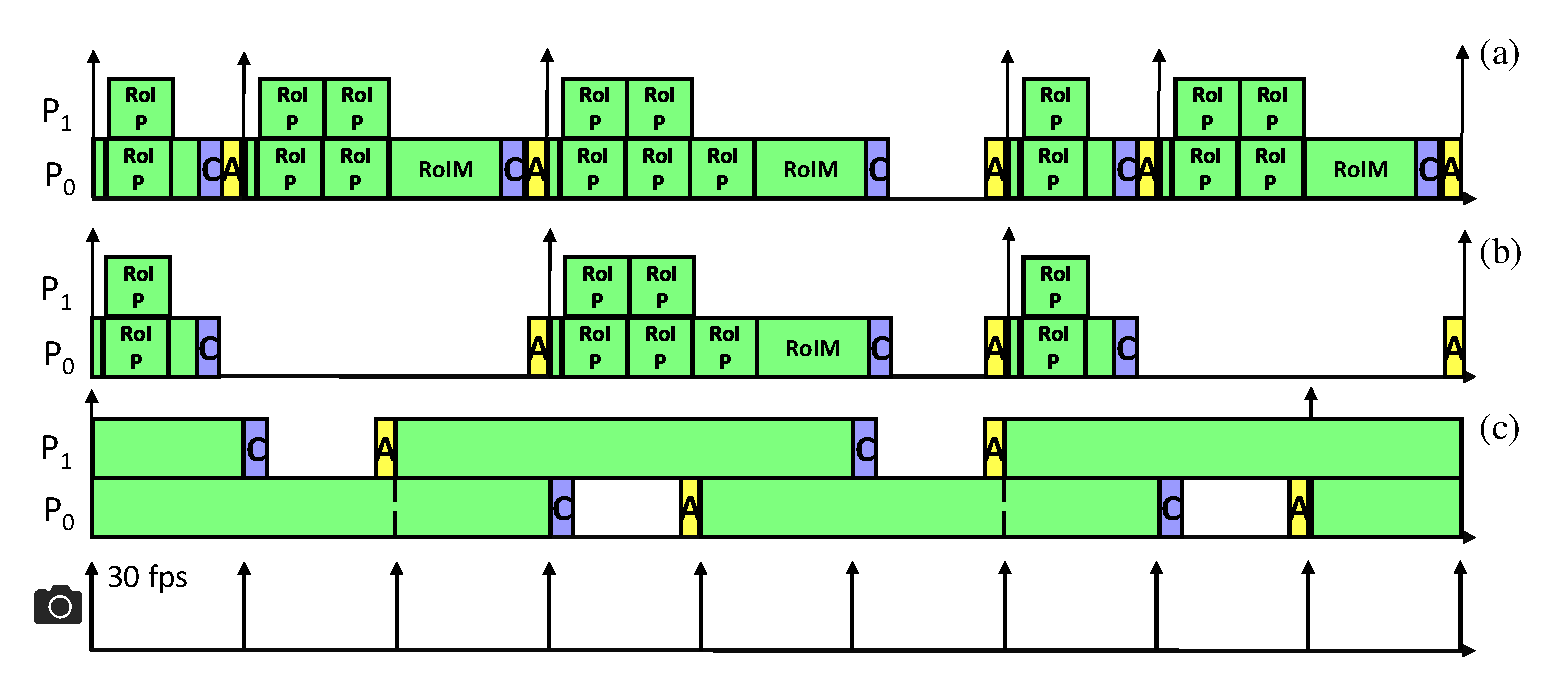
\includegraphics[scale=0.5]{images/results_gantt.eps}}
            \vspace{-1ex}
            \caption{Gantt charts for (a) switching sequence $(s_1 s_2 s_{wc})^\omega$, (b) corresponding worst-case design $(s_{wc})^\omega$, and (c) pipelined control design used for comparison.}
            \label{fig:ch5_result2}
            \vspace{-2ex}
        \end{figure}

\subsection{Comparison with state-of-the-art pipelined control}
We compare our \gls{spade} approach with a state-of-the-art pipelined control approach~\cite{medina2019designing}. For fairness in the comparison, we use the same control design technique - \gls{lqr} with integral action - explained in~\cite{medina2019designing} for \gls{spade}.  
Further, we consider the same given platform allocation of two processors. 
\\[1ex]
\noindent\textbf{Pipelined control design:} 
We discretize the continuous-time system model in Eq.~(\ref{eq:ch5_ch5_contsys}) with sensor-to-actuator delay $\tau$ and sampling period $h$ to obtain a delayed input system,
\begin{eqnarray}
\label{eq:ch5_disc_sys_parallel}
x((k+1)h) = \Adyn x(kh)+\Bdyn u(kh-h),
\end{eqnarray}
where $\Adyn,\ \Bdyn$ are the discretized state and input matrices respectively. 
Here, $\Adyn=e^{\Acont h}$ and  $\Bdyn=\int_{0}^{h} e^{\Acont s} \Bcont ds$.
The control input $u(t)$ applied at $t = kh$
uses $h$ time units old sensing information in
any sampling interval $kh$ to $(k + 1)h$ due to the sensor-to-actuator delay $\tau$. This is reflected in Eq.~(\ref{eq:ch5_disc_sys_parallel}) as the delayed
input $u(kh-h)$.

For brevity, the pipelined control delay and period is represented as $\tau$ and $h$ in this subsection. $\tau=\lceil\frac{\actorET_{\text{total}}}{\fh}\rceil \fh$ and $h=\frac{\tau}{\gamma}$, where $\gamma$ is the number of processing cores. Note that in~\cite{medina2019designing}, there is a strict criterion that the sampling period should be an integral multiple of $\fh$ and strictly periodic. As such the $\tau$ should be relaxed based on $\gamma$. E.g., in our \gls{lkas} case, if $\actorET_{\text{total}}=0.084$s, we get $\tau=0.100$s and $h=0.050$s for $\gamma=2$. However, $h=0.050$s is not an integral multiple of $\fh$ and as such we have to relax $\tau$ so that $\tau=0.100+\fh=0.133$s and $h=0.067$s which is an integral multiple of $\fh$. 

For designing the delayed control input $u(kh-h)$, one
design option is to transform the system in Eq.~(\ref{eq:ch5_disc_sys_parallel}) into standard non-delayed
form and apply any standard control design technique.
Towards this, we define a new system state vector $\hat{z}(kh)=\left[ \begin{array}{cc} x^T(kh) &  u(kh-h) \end{array} \right]^T$ to obtain a higher-order augmented system in the non-delayed form as follows:
\begin{eqnarray}
\label{eq:ch5_aug_pipelined}
\hat{z}(kh+h) &= \Phi_d\hat{z}(kh) + \Gamma_du(kh) \\
y(kh) &= \Cdyn \hat{z}(kh),\nonumber
\end{eqnarray}
where $\Phi_d,\ \Gamma_d,\ \Cdyn$ are the augmented discretized matrices such that,
\begin{eqnarray}
\Phi_d = \left[ \begin{array}{ccc} \Adyn &  \Bdyn & \bm{0} \\  \bm{0} & \bm{0} & \bm{I} \\
\bm{0} & \bm{0} & \bm{0}\end{array} \right],\
\Gamma_{d} = \left[ \begin{array}{c} \bm{0} \\ \bm{0} \\ 1  \end{array} \right].
\nonumber
\end{eqnarray}
$\bm{0}$ and $\bm{I}$ represent the zero and identity matrices of appropriate dimensions. A check for controllability~\cite{dorf2011modern} is done for this augmented system.
If the system is not controllable, controllability decomposition is done to obtain a controllable subsystem.

The system in Eq.~(\ref{eq:ch5_aug_pipelined}) is in standard discrete-time form for which a standard discrete-time control design technique such as \gls{lqr}~\cite{dorf2011modern} can be used.
We use an \gls{lqr}-based optimal state feedback controller, with integral action for reference tracking, referred to in literature as \gls{lqi} control~\cite{zhou1996robust,young1972approach}. The state feedback controller is of the form,
\begin{eqnarray}
u(kh)=\Kgain \left[ \begin{array}{c} \hat{z}(kh) \\ x_i(kh)  \end{array} \right],\text{ where }x_i(kh+h)=x_i(kh)+y(kh)-r(kh).
\label{eq:ch5_LQI_u}
\end{eqnarray}
$\Kgain$ is the \gls{lqr} state feedback gain designed for the state space considering the integral action as given below,
\begin{eqnarray}
\left[ \begin{array}{c}\hat{z}(kh+h)\\x_i(kh+h)  \end{array} \right] &= \left[ \begin{array}{cc}\Phi_d & \bm{0}\\C_d & \bm{1}  \end{array} \right]\left[ \begin{array}{c}\hat{z}(kh)\\x_i(kh)  \end{array} \right] + \left[ \begin{array}{c}\Gamma_d\\\bm{0}  \end{array} \right] u(kh).
\label{eq:ch5_LQI_ss}
\end{eqnarray}
This control design replaces the earlier presented \gls{lqr} control design for each scenario in \gls{spade}. We do so to have a fair comparison between different implementation strategies since the control theory for pipelined control systems considers that $\tau$ and $h$ are integral multiples of $\fh$. However, the controller design approach of \gls{spade} can have any value for $\tau$ and hence is more flexible than pipelined control. 
We adapt the pipelined control design applicable for $\tau\ge h$ to the \gls{spade} approach applicable for any $\tau<h$ by modifying Eq.~(\ref{eq:ch5_LQI_ss}) with parameters from Eq.~(\ref{eq:ch5_ch5_cld2}):
\begin{eqnarray}
\left[ \begin{array}{c}\hat{z}(kh+h)\\x_i(kh+h)  \end{array} \right] &= \left[ \begin{array}{cc}\Aaugs & \bm{0}\\ \Caug & \bm{1}  \end{array} \right]\left[ \begin{array}{c}\hat{z}(kh)\\x_i(kh)  \end{array} \right] + \left[ \begin{array}{c}\Baugs \\\bm{0}  \end{array} \right] u(kh).
\nonumber
\end{eqnarray}
Then, we design the gain $\Kgain_{\sysScenario}$ for each \gls{spade} scenario $\sysScenario$ using  Eq.~(\ref{eq:ch5_LQI_u}).
\\[1ex]
\noindent\textbf{Comparison:}
For pipelined control, the total sensor-to-actuator delay $\actorET_{\text{total}}= 5 + 6\times 10+6\times 7+2+2=111$ms (since each pipe executes sequentially), the effective sensor-to-actuator delay = $\tau=\lceil \frac{\actorET_{\text{total}}}{\fh}\rceil \fh= 133.33$ms, and the sampling period $h=\frac{\tau}{2}=66.67$ms for the given two processing cores. The Gantt chart of the pipelined execution is shown in Fig.~\ref{fig:ch5_result2}(c). As mentioned, for \gls{spade}, we use the same pipelined control design approach. For scenario $s_{wc}$, $\actorET_{\text{total}}=5+3\times 10+6\times 7+2+2=81$ms so that $\tau_{s_{wc}}=0.100=h_{wc}$. Similarly, for scenario $s_1$, $\tau_1=0.033=h_1$ and for scenario $s_2$,   $\tau_2=0.067=h_2$.

\begin{figure}[t]
            \centerline{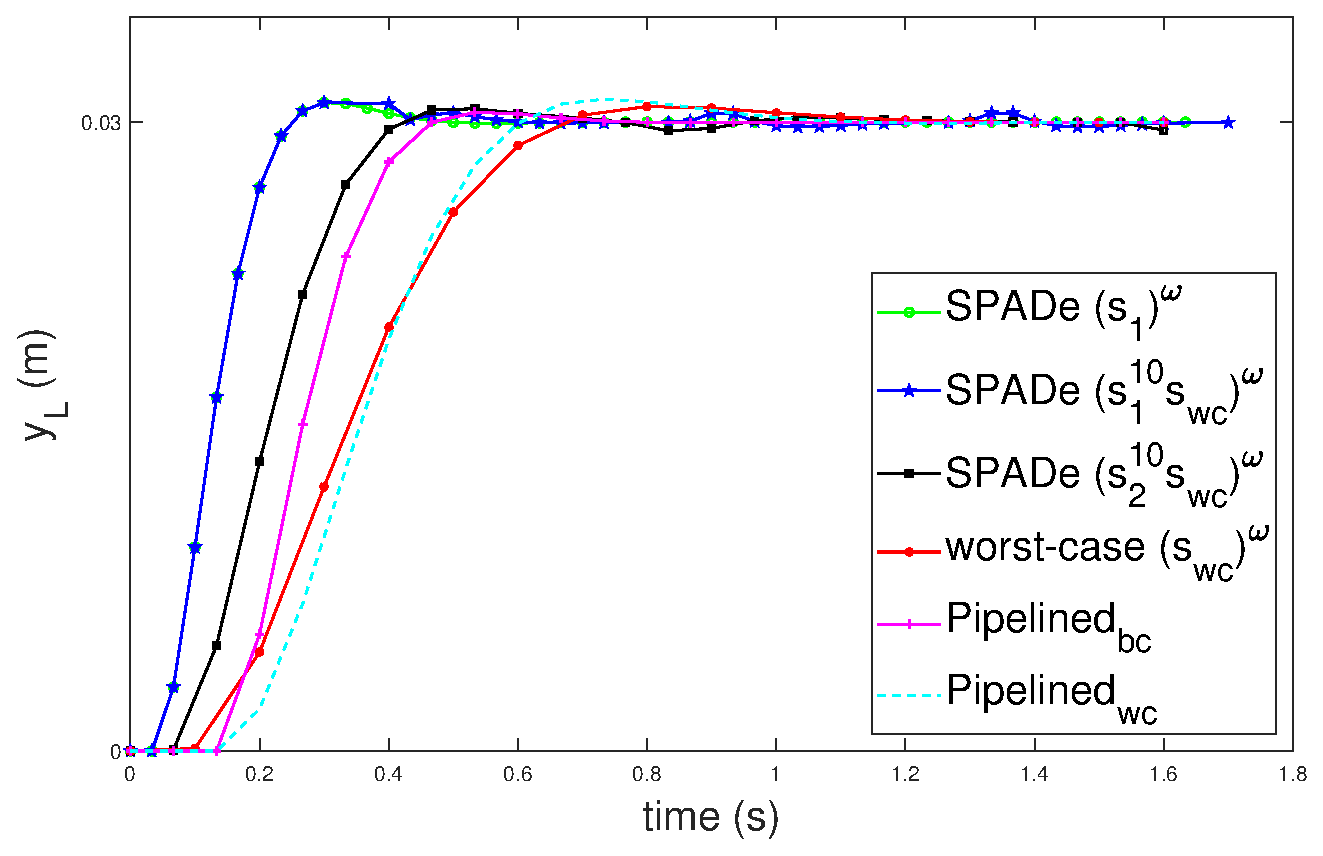
\includegraphics[scale=0.5]{images/res_fig10.eps}}
            \vspace{-1ex}
            \caption{Comparison between pipelined and \gls{spade} approach}
            \label{fig:ch5_comparison}
            %\vspace{-4ex}
\end{figure}

The results of the comparison between the pipelined controller with respect to the \gls{spade} approach are shown in Fig.~\ref{fig:ch5_comparison}. 
Note that \gls{spade} allows for parallelisation that reduces both sampling period and sensor-to-actuator delay. 
However, pipelining only reduces the sampling period.

The key observations are:
\begin{itemize}
    \item The performance of the \gls{lqi} controllers highly depends on the quality of controller tuning~\cite{medina2019designing}. We observe that the \gls{qoc} of the pipelined controller is always in the range of \gls{qoc} between the worst-case design and the \gls{spade} approach. Fig.~\ref{fig:ch5_comparison} shows two different tunings of the pipelined controller: plot pipelined\textsubscript{bc} is tuned with the same control parameters as scenario $s_1$ and pipelined\textsubscript{wc} is tuned with the same control parameters as scenario $s_{wc}$.
    
If we execute in a frequently occurring scenario, e.g., $s_1$ (see plot $(s_1^{10}s_{wc})^\omega$ in Fig.~\ref{fig:ch5_comparison}), then we see that the control performance is better than the pipelined control. In this particular case, arbitrary switching between $s_1,\ s_2,$ and $s_{wc}$ is unstable. To meaningfully apply the \gls{spade} approach, we should have a frequently occurring scenario during run time, and switching from this frequently occurring scenario to the worst-case should be stable, e.g., based on a dwell time criterion~\cite{12_sunstability} (as shown for plots $(s_1^{10}s_{wc})^\omega$ and $(s_2^{10}s_{wc})^\omega$ in Fig.~\ref{fig:ch5_comparison}).
\item \gls{spade} performs better with a shorter $\tau$ when $\tau<h$ and other control tuning parameters are kept the same. When $\tau_1<\tau_2<h$, the case with $\tau_1$ will have better performance than $\tau_2$ for the same $h$.  The actual performance improvement further depends on the system dynamics.
\end{itemize}

\gls{spade} gives prominent advantages when the algorithm structure is known, i.e., the application is a white/gray box and when there is scope for parallelisation.
Pipelining works also when the application is a black box and is not dependent on the parallelisation of the algorithm. However, pipelining cannot be used when there are inter-frame dependencies for the algorithm, whereas \gls{spade} is not affected by  inter-frame dependencies (as further elaborated in the next two chapters).
Further, \gls{spade} gives better results when the application is executing in its frequently occurring scenario. Pipelining is better suited if the application is frequently executing closer to its worst case. A brief comparison between \gls{spade} and pipelined approaches is illustrated in Table~\ref{table:comparison}. In the following two chapters, we integrate pipelining in \gls{spade}, effectively combining the advantages of the two approaches.

\begin{table}
\scriptsize
\caption{\gls{spade} vs pipelined: applicability criteria and comparison}
\label{table:comparison}
\vspace{-1em}
\centering
\begin{tabular}{|l|l|l|ll}
\cline{1-3}
\multicolumn{1}{|c|}{Criteria} & \multicolumn{1}{c|}{\gls{spade}}         & \multicolumn{1}{c|}{Pipelining~\cite{medina2019designing}} &  &  \\ \cline{1-3}
Algorithm       & should be white/gray box & white/gray/black box                               &  &  \\ \cline{1-3}
Degree of parallelisation & should be high for better \gls{qoc}                                & independent (no parallelism)  &  &  \\ \cline{1-3}               Inter-frame dependencies  & independent (no pipelining) & should not exist \\ \cline{1-3}
Workload variations                               & considered in design                                   &                   not considered              &  &  \\ \cline{1-3}
Platform                               & independent (applicable for all)                                   &                   suitable mainly for homogeneous              &  &  \\ \cline{1-3}
Restrictions on $h$                                & any multiple of $\fh$                                   &                   multiple of $\fh$; strictly periodic              &  &  \\ \cline{1-3}
Restrictions on $\tau$                                & none                                   &                   multiple of $h$ and $(\gamma\times \fh)$      &  &  \\ \cline{1-3}
\end{tabular}
\end{table}